\newcommand{\sfs}{\fontsize{14pt}{15pt}\selectfont}
\sfs % размер шрифта и расстояния между строками
\thispagestyle{empty}

\vspace{5mm}
\begin{flushright}
  \LargeНа правах рукописи
\end{flushright}

\begin{figure}[h!] 
\begin{flushright}
  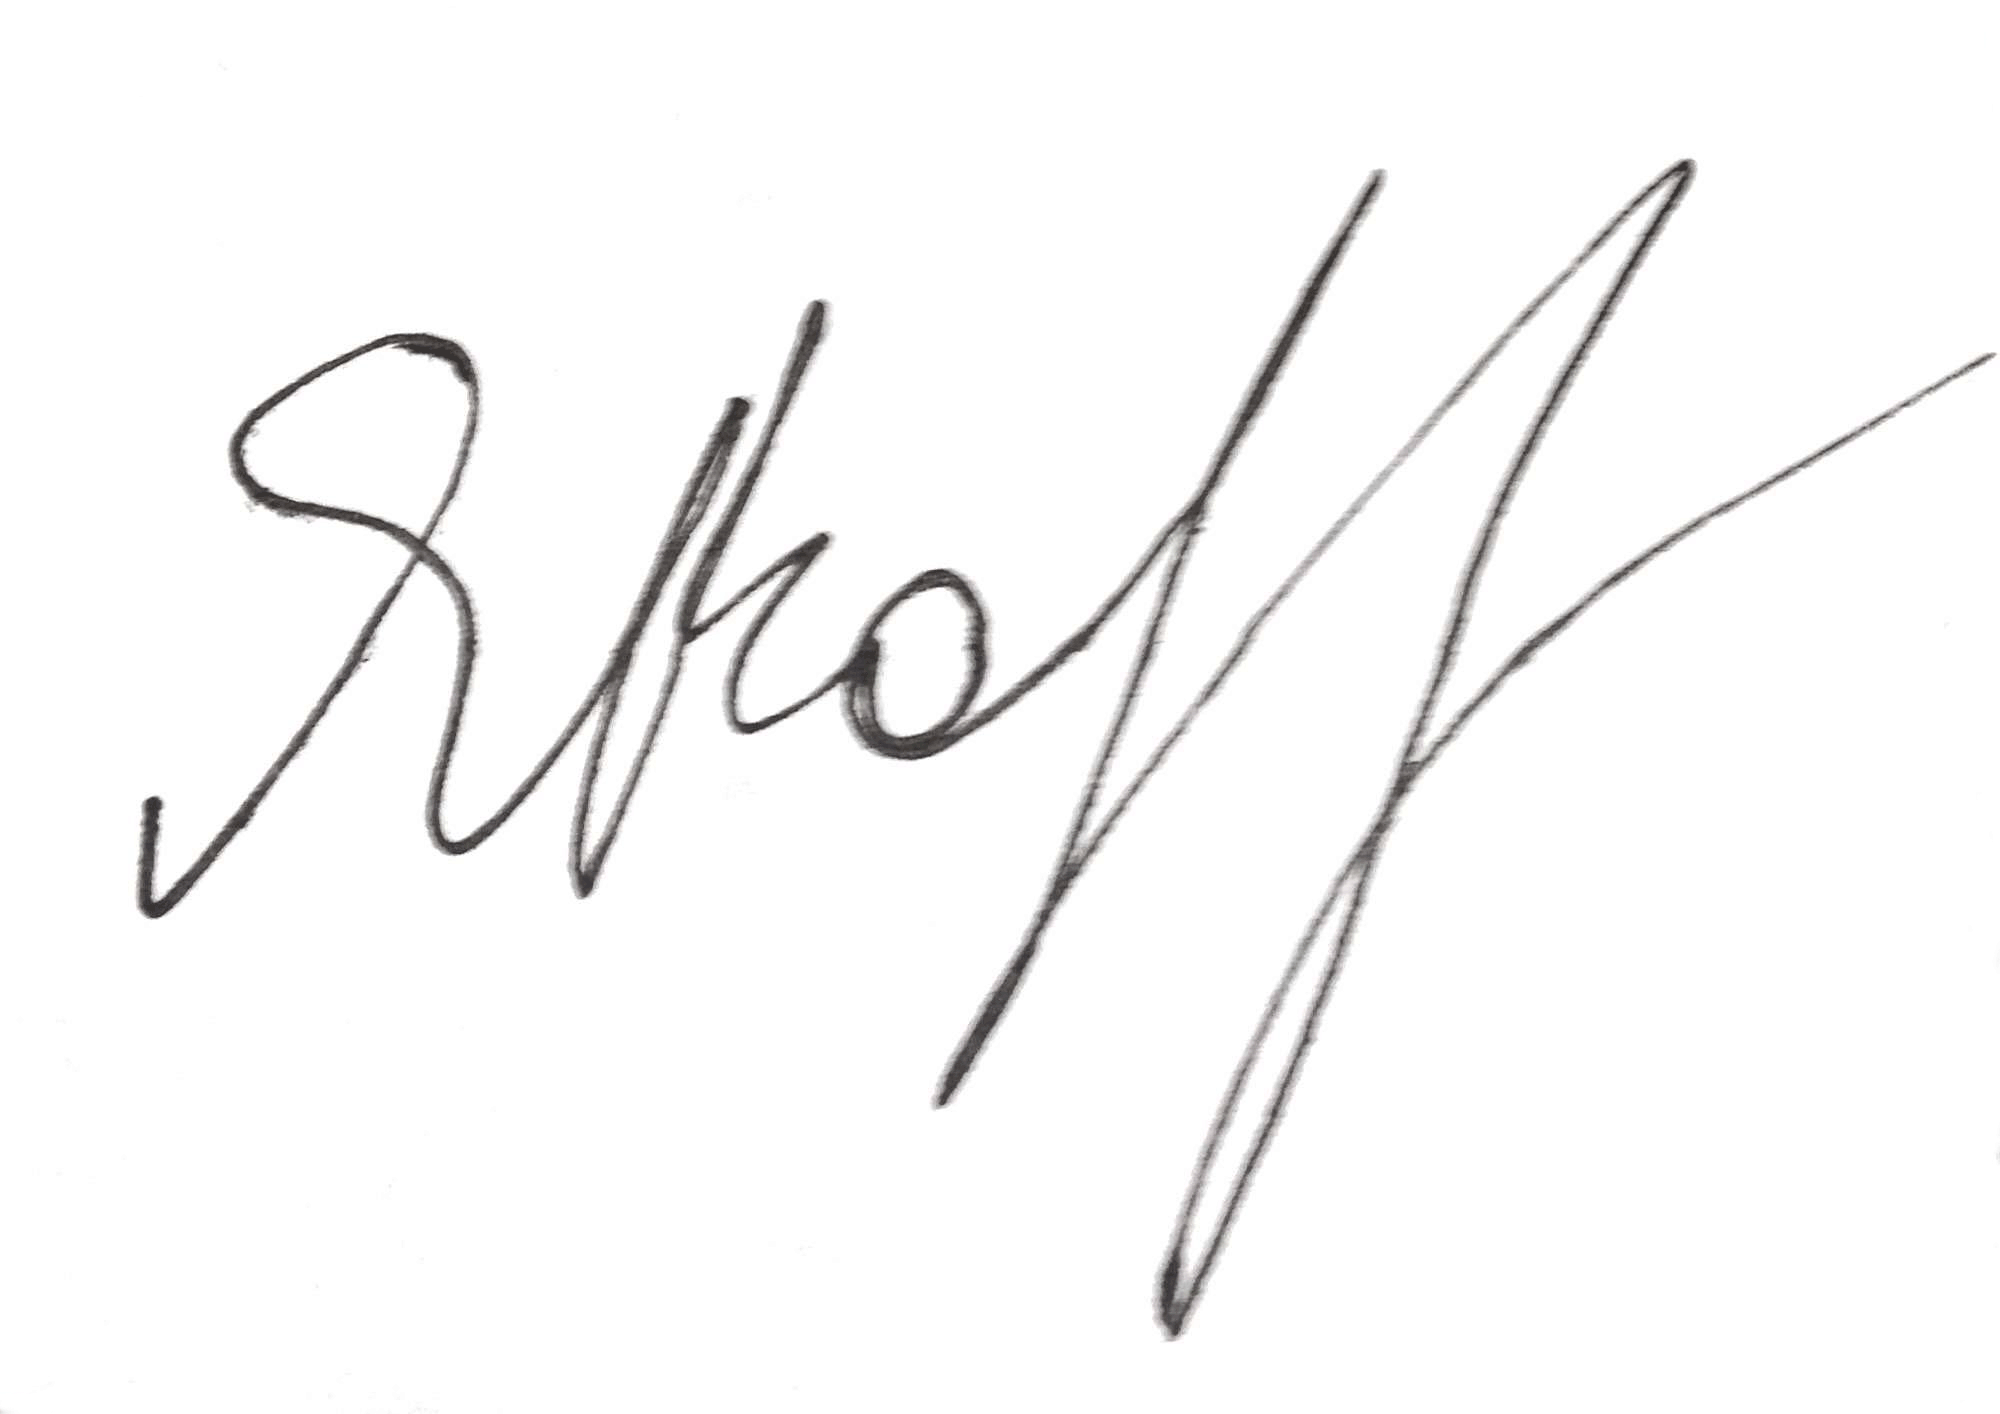
\includegraphics[width=4cm]{signature-mine.png}
\end{flushright}
\end{figure}

\vspace{5mm}
\begin{center}
{\Large\bf Воронцов Ярослав Александрович}
\end{center}

\vspace{15mm}
\begin{center}
{\bf \LARGE \MakeUppercase {Математическое моделирование задач выбора с расплывчатой неопределенностью на основе методов представления и алгебры нечетких параметров}
\par}

\vspace{20mm}
{\Large
05.13.18~--- математическое моделирование, численные методы\par и комплексы программ
}

\vspace{15mm}
\textbf{Автореферат}\par
\Largeдиссертации на соискание учёной степени\par
кандидата физико-математических наук
\end{center}

\vspace{40mm}
\begin{center}
{\LargeВоронеж --- 2015}
\end{center}

\newpage
% оборотная сторона обложки
\thispagestyle{empty}
\noindent Работа выполнена в Федеральном государственном бюджетном образовательном учреждении высшего профессионального образования <<Воронежский государственный университет>>

\vspace{10mm}

\begin{table} [h]  
  \begin{tabular}{ll}  
   \makecell[l]{\sfs Научный руководитель:\\~} &
   \makecell*[{{p{11cm}}}]{
   \sfs доктор технических наук, профессор\\
   \textbf{\sfs Матвеев Михаил Григорьевич}
   }
      
\vspace{5mm} \\

   \makecell[l]{\sfs Официальные оппоненты: \vspace{4.4cm}} &
   \makecell[{{p{11cm}}}]{   
   \sfs \textbf{Блюмин Семён Львович,} \\
   \sfs доктор физико-математических наук, профессор, \\
   \sfs Липецкий государственный технический университет,
   кафедра прикладной математики, профессор \vspace{3mm} \\ 
   \sfs \textbf{Анисимов Дмитрий Николаевич,} \\
   \sfs кандидат технических наук, доцент, \\
   \sfs Московский энергетический институт, \\
   \sfs кафедра управления и информатики, доцент
   }

\vspace{5mm} \\

   \makecell[l]{\sfs Ведущая организация:} &
   \makecell*[{{p{11cm}}}]{\sfs
   Тверской государственный технический университет
   }
  \end{tabular}  
\end{table}

\vspace{20mm} Защита состоится <<\ \ \ >> апреля 2015~г.~в~XX часов на~заседании диссертационного совета Д.212.038.020 при Федеральном государственном бюджетном образовательном учреждении высшего профессионального образования <<Воронежский государственный университет>> по адресу: 394006, г.~Воронеж, Университетская пл., д.\,1, ауд. 335.

\vspace{5mm}
\noindent С диссертацией можно ознакомиться в научной библиотеке Воронежского государственного университета и на сайте http://www.science.vsu.ru/disser.

\vspace{5mm}
\noindentАвтореферат разослан <<\ \ \ >> марта 2015 года.

\vspace{10mm}
\begin{table} [h]
  \begin{tabular}{p{8cm}r}
    \begin{tabular}{p{8cm}}
      \sfs Ученый секретарь  \\
      \sfs диссертационного совета  \\
      \sfs кандидат физико-математических наук
      \sfs доцент
    \end{tabular}
    & \begin{tabular}{r}
       \\
       \\
       \sfs    \hspace{50mm}  Шабров С.А.
    \end{tabular} 
  \end{tabular}
\end{table}
\newpage